\documentclass[12pt,a4paper]{article}

\usepackage[a4paper,margin=1in]{geometry}
\usepackage{graphicx}
\usepackage{booktabs}
\usepackage{amsmath,amssymb}
\usepackage{float}
\usepackage{hyperref}
\usepackage{xcolor}
\usepackage{listings}
\usepackage{enumitem}
\usepackage{fancyhdr}
\usepackage{longtable}
\usepackage{subcaption}   % required for the 2-graphs-per-row layout
\usepackage{mathptmx}     % Times New Roman substitute font (text + math)
\usepackage{fontawesome} % for using icons

\hypersetup{colorlinks=true,linkcolor=blue,urlcolor=blue}

\pagestyle{fancy}
\fancyhf{}
\lhead{ICS1512}
\rhead{Machine Learning Algorithms Laboratory}
\cfoot{\thepage}

\lstset{
language=Python,
basicstyle=\ttfamily\small,
numbers=left,
frame=single,
breaklines=true,
showstringspaces=false
}

\begin{document}

\begin{tabular}{|p{4cm}|p{11cm}|}
\hline
Experiment No. & 4\\ \hline
Experiment Title &  Binary Classification using Linear and Kernel-Based Models \href{https://github.com/Poojashree81/ICS1512-Machine-Learning-Laboratory.git}{\faGithub} \\ \hline
Student Name & Poojashree V \\ \hline
Register Number & 3122247001043 \\ \hline
Faculty & Dr. Poreddy Ajay Kumar Reddy \\ \hline
Submission Date & 28th July 2026\\ \hline
\end{tabular}

\section{Objective}
This experiment builds and compares two binary classifiers -- Logistic Regression and
Support Vector Machine (SVM) -- for detecting spam emails on the Spambase dataset. We
also look at how hyperparameter tuning (Grid Search with 5-fold cross-validation)
affects the regularization behaviour of Logistic Regression and shapes the
kernel-induced decision boundary of SVM. Each tuned model is then evaluated on
accuracy, precision, recall, F1-score, training time, and cross-validated stability,
and we try to draw some practical conclusions about the accuracy--complexity--interpretability
trade-off between a linear probabilistic model and a margin-based kernel model.
 
\section{Problem Statement}
Given 4601 emails represented by 57 numerical features (word-frequency percentages,
character-frequency percentages, and statistics of consecutive capital-letter runs),
the task is to predict a binary label -- \texttt{class = 1} for spam and
\texttt{class = 0} for non-spam (ham). The input is the standardized 57-dimensional
feature vector for each email; the output is the predicted class label (and, where
supported, a class-membership probability). What we're really after is which of the
two model families -- a linear, probabilistically-calibrated classifier (Logistic
Regression) or a margin-based, kernel-transformable classifier (SVM) -- generalizes
best to unseen emails once hyperparameters are tuned, while still keeping an eye on
training cost and interpretability.
 
\section{Dataset Description}
\begin{longtable}{|p{6cm}|p{8cm}|}
\hline
Dataset Name & Spambase \\ \hline
Dataset Source & Kaggle (\texttt{somesh24/spambase}), originally hosted on the UCI
Machine Learning Repository \\ \hline
Number of Samples & 4601 emails \\ \hline
Number of Features & 57 numeric features (48 word-frequency, 6 character-frequency,
3 capital-run-length statistics) \\ \hline
Number of Classes & 2 (0 = ham/non-spam, 1 = spam) \\ \hline
Missing Values & None -- \texttt{df.isnull().sum()} returned 0 for all 58 columns;
a mean-strategy \texttt{SimpleImputer} was still applied defensively before scaling \\ \hline
Train-Test Split & 80:20 (3680 training samples / 921 test samples),
\texttt{random\_state=42} \\ \hline
\end{longtable}
 
\section{Exploratory Data Analysis}
\begin{itemize}
\item Dataset overview -- \texttt{df.head()} and \texttt{df.info()} confirmed 4601
rows $\times$ 58 columns, all of \texttt{float64}/\texttt{int64} dtype, with the last
column (\texttt{class}) as the binary target.
\item Statistical summary -- \texttt{df.describe()} showed heavily right-skewed
word-frequency and character-frequency columns (most medians sitting at 0, with long
right tails and some fairly large maxima), and a capital-run-length feature set with
very high variance (std $\approx$ 31.7 for \texttt{capital\_run\_length\_average},
with max run lengths reaching several hundred characters).
\item Missing value analysis -- we verified 0 missing values across all 58 columns
before any imputation was applied.
\item Class distribution -- see Figure~\ref{fig:class-dist}.
\item Correlation matrix -- see Figure~\ref{fig:corr-heatmap}.
\item Feature distribution -- we didn't generate a separate per-feature histogram grid
in this run; the \texttt{describe()} summary above was used instead to get a sense of
feature skew.
\end{itemize}
 
\begin{figure}[H]
\centering

\includegraphics[width=0.55\linewidth]{figures/class_distribution.eps}
\caption{Class distribution of the Spambase dataset (0 = ham, 1 = spam).}\label{fig:class-dist}
\end{figure}
 
\textbf{Inference:} 
From Figure~ \ref{fig:class-dist} we can see a moderate class imbalance, with non-spam
(ham) emails making up the majority class -- this lines up with the dataset's
well-documented roughly 60:40 ham-to-spam split. Since the imbalance isn't extreme
(nowhere near, say, 95:5), plain accuracy is still a reasonably informative metric on
its own, but we tracked precision and recall separately anyway, just to make sure the
minority spam class wasn't getting misclassified disproportionately. This class ratio
is also why we used stratifiable cross-validation folds during hyperparameter search
rather than leaning on a single train-test split. One possible explanation for why
recall on the spam class (0.874) trailed precision (0.932) for the baseline Logistic
Regression model is exactly this imbalance. Overall, the distribution suggests the
dataset is fine for standard binary classification metrics without needing resampling
tricks like SMOTE.
 
\begin{figure}[H]
\centering
\includegraphics[width=0.75\linewidth]{figures/correlation_heatmap.eps}
\caption{Pairwise Pearson correlation heatmap across all 58 columns of the Spambase dataset.}\label{fig:corr-heatmap}
\end{figure}
 
\textbf{Inference:}
Looking at Figure~ \ref{fig:corr-heatmap}, the heatmap is mostly cool, near-zero
correlations across the word-frequency features, which suggests individual word
occurrences are largely independent of one another -- not too surprising for a
bag-of-words-style representation where any given word tends to be rare in any single
email. A few warmer clusters do show up among semantically related features, like the
character-frequency group (\texttt{char\_freq\_\%28}, \texttt{char\_freq\_\%21},
\texttt{char\_freq\_\%24}) and the three \texttt{capital\_run\_length\_*} columns,
which co-vary because emails with long runs of capital letters tend to have both a
higher average and a higher longest run. There's no strong multicollinearity here (no
near-1 off-diagonal blocks outside these small clusters), which tells us aggressive
dimensionality reduction probably wasn't necessary before modeling, and that letting
L1-regularized Logistic Regression handle feature selection itself (rather than
reaching for PCA) was a reasonable call. This also helps explain why Grid Search
ended up preferring an $\ell_1$ penalty for Logistic Regression: with so many
near-independent, low-information word-frequency columns floating around, driving the
redundant coefficients to exactly zero improves generalization.
 
\section{Data Preprocessing}
 
\begin{itemize}
\item \textbf{Missing value handling:} A \texttt{SimpleImputer(strategy="mean")} was
fit on all 57 feature columns. Since the dataset had zero missing values to begin
with, this step had no real numerical effect, but we kept it in as a defensive
measure.
\item \textbf{Encoding:} Not needed -- all 57 input features are continuous numeric
frequencies/statistics, and the target \texttt{class} is already encoded as 0/1.
\item \textbf{Feature scaling:} A \texttt{StandardScaler} was fit exclusively on
\texttt{X\_train} and then used to transform both \texttt{X\_train} and
\texttt{X\_test}, giving zero-mean, unit-variance features. This step really matters
for both models here: Logistic Regression's regularization penalty is scale-sensitive,
and SVM's RBF/polynomial/sigmoid kernels compute distances/inner products that get
distorted if the features aren't scaled.
\item \textbf{Train-test split:} \texttt{train\_test\_split} was used with
\texttt{test\_size=0.2} and \texttt{random\_state=42}, giving 3680 training and 921
test samples. The scaler was fit only after the split, to avoid leaking any
information from the test set.
\item \textbf{Feature engineering:} None beyond scaling -- we used the original 57
Spambase features (word-frequency \%, character-frequency \%, and capital-run-length
statistics) directly.
\end{itemize}
 
\section{Machine Learning Algorithm}
 
\subsection*{Logistic Regression}
\begin{itemize}
\item \textbf{Working principle:} Logistic Regression models the log-odds of the
positive class as a linear combination of the input features and squashes this score
through the sigmoid function to obtain a probability, $P(y=1\mid x) = \frac{1}{1 +
e^{-(w^Tx+b)}}$. A decision threshold (0.5 by default) then converts this probability
into a class label.
\item \textbf{Mathematical formulation:} The weights $w$ and bias $b$ are learned by
minimizing the regularized log-loss,
\[
J(w,b) = -\frac{1}{n}\sum_{i=1}^{n}\Big[y_i\log(\hat{p}_i) + (1-y_i)\log(1-\hat{p}_i)\Big]
+ \frac{1}{C}\,R(w),
\]
where $\hat p_i = \sigma(w^Tx_i+b)$, $C$ is the inverse regularization strength, and
$R(w)$ is either the $\ell_1$ norm $\lVert w \rVert_1$ (Lasso -- drives coefficients to
exactly zero, useful for feature selection) or the $\ell_2$ norm $\lVert w \rVert_2^2$
(Ridge -- shrinks all coefficients smoothly without eliminating them).
\item \textbf{Advantages:} Quick to train (0.030\,s here), naturally probabilistic
outputs, coefficients that are easy to interpret, and low variance -- makes for a
solid baseline model.
\item \textbf{Limitations:} It assumes a linear decision boundary in feature space, so
it can't capture the kind of non-linear feature interactions that, in this
experiment, the RBF kernel was able to exploit for a small extra bump in accuracy.
\end{itemize}
 
\subsection*{Support Vector Machine (SVM)}
\begin{itemize}
\item \textbf{Working principle:} SVM finds the hyperplane that maximizes the margin
between the two classes; only the training points closest to the boundary (the
support vectors) actually determine where that boundary sits. Using the kernel
trick, SVM can implicitly map inputs into a higher-dimensional space, which lets it
separate classes that aren't linearly separable in the original feature space.
\item \textbf{Mathematical formulation:} The primal soft-margin objective is
\[
\min_{w,b,\xi}\ \tfrac{1}{2}\lVert w \rVert^2 + C\sum_{i=1}^{n}\xi_i
\quad \text{s.t.}\quad y_i(w^T\phi(x_i)+b) \ge 1-\xi_i,\ \xi_i \ge 0,
\]
where $\phi(\cdot)$ is the (implicit) kernel feature map. We compared four kernels in
this experiment: linear $K(x_i,x_j)=x_i^Tx_j$; polynomial
$K(x_i,x_j)=(\gamma x_i^Tx_j + r)^d$; RBF $K(x_i,x_j)=\exp(-\gamma\lVert x_i-x_j\rVert^2)$;
and sigmoid $K(x_i,x_j)=\tanh(\gamma x_i^Tx_j + r)$.
\item \textbf{Advantages:} The RBF kernel picked up on non-linear structure in the
standardized feature space and ended up with the highest test accuracy of every
model/kernel we evaluated (93.49\%). SVMs also tend to hold up reasonably well
against overfitting in high-dimensional feature spaces once $C$ and $\gamma$ are
tuned.
\item \textbf{Limitations:} Noticeably slower to train than Logistic Regression
(1.7--2.7\,s per kernel here versus 0.03\,s), no native probability output (you'd need
Platt scaling via \texttt{probability=True}, which adds further overhead), harder to
interpret than a linear model's coefficients, and -- as this experiment's polynomial
kernel result makes clear (76.66\% accuracy) -- quite sensitive to a poor
kernel/hyperparameter choice.
\end{itemize}
 
\section{Experimental Setup}
\begin{tabular}{ll}
\toprule
Python Version & 3.12 \\
Scikit-Learn Version & 1.6.1 \\
IDE & Jupyter Notebook \\
Operating System & Linux (Ubuntu-based) \\
Hardware & CPU \\
\bottomrule
\end{tabular}
 
\section{Hyperparameter Selection}
 
\subsection*{Logistic Regression search space}
\begin{tabular}{ll}
\toprule
Parameter & Values searched\\
\midrule
Penalty & $\{$l1, l2$\}$ \\
$C$ (inverse regularization strength) & $\{0.01,\ 0.1,\ 1,\ 10,\ 100\}$ \\
Solver & $\{$liblinear, saga$\}$ \\
\bottomrule
\end{tabular}
 
\subsection*{SVM search space}
\begin{tabular}{ll}
\toprule
Parameter & Values searched\\
\midrule
Kernel & $\{$linear, poly, rbf, sigmoid$\}$ \\
$C$ & $\{0.1,\ 1,\ 10,\ 100\}$ \\
$\gamma$ & $\{$scale, auto$\}$ \\
\bottomrule
\end{tabular}
 
Both models were tuned using \texttt{GridSearchCV} with 5-fold cross-validation on
the training set only ($X_{train}$, $y_{train}$).
 
\section{Hyperparameter Tuning Results}
 
\begin{tabular}{lp{4cm}p{5cm}c}
\toprule
Model & Search Method & Best Parameters & Best CV Accuracy\\
\midrule
Logistic Regression & Grid Search & $C=10$, penalty=l1, solver=liblinear & 0.9274 \\
SVM & Grid Search & $C=1$, $\gamma$=scale, kernel=rbf & 0.9307 \\
\bottomrule
\end{tabular}
 
Grid Search ended up preferring an $\ell_1$-penalized Logistic Regression with a
relatively large $C=10$ (weak regularization), which basically means most of the 57
features were still informative enough to keep, with sparsity only trimming away the
least useful ones. For SVM, the RBF kernel with the default \texttt{scale} $\gamma$
(i.e. $\gamma = 1 / (57 \times \text{Var}(X))$) and a moderate $C=1$ beat out every
other kernel/parameter combination in cross-validation, edging past the tuned
Logistic Regression by about 0.33 percentage points in CV accuracy.
 
\section{Results}
 
\subsection*{Logistic Regression Performance (baseline model, default $C=1$, L2 penalty)}
\begin{tabular}{lc}
\toprule
Metric & Value\\
\midrule
Accuracy & 0.9197 \\
Precision & 0.9317 \\
Recall & 0.8744 \\
F1-score & 0.9021 \\
ROC-AUC & Not computed \\
Training Time (s) & 0.0301 \\
\bottomrule
\end{tabular}
 
\subsection*{SVM Kernel-wise Performance}
\begin{tabular}{lcccc}
\toprule
Kernel & Accuracy & F1 Score & Training Time (s)\\
\midrule
Linear & 0.9262 & 0.9105 & 2.5546 \\
Polynomial & 0.7666 & 0.6337 & 2.7196 \\
RBF & 0.9349 & 0.9206 & 1.6794 \\
Sigmoid & 0.8762 & 0.8500 & 1.7296 \\
\bottomrule
\end{tabular}
 
\subsection*{Final Tuned-Model Comparison (test set)}
\begin{tabular}{lcc}
\toprule
Model & Accuracy & Training Time (s)\footnote{As coded in the notebook, this column
reports the time to fit the initial, untuned baseline of each model family (default
Logistic Regression and the linear-kernel SVC respectively) rather than a separate
timing run for the grid-search-selected estimator; it is reproduced here exactly as
computed for record accuracy.}\\
\midrule
Logistic Regression (tuned: L1, $C=10$) & 0.9164 & 0.0301 \\
SVM (tuned: RBF, $C=1$, $\gamma$=scale) & 0.9349 & 0.6281 \\
\bottomrule
\end{tabular}
 
\subsection*{K-Fold Cross-Validation Results ($K=5$, on training set)}
\begin{tabular}{ccc}
\toprule
Fold & Logistic Regression & SVM\\
\midrule
Fold 1 & 0.9375 & 0.9348 \\
Fold 2 & 0.9049 & 0.9049 \\
Fold 3 & 0.9334 & 0.9402 \\
Fold 4 & 0.9307 & 0.9375 \\
Fold 5 & 0.9307 & 0.9361 \\
\midrule
Average & 0.9274 & 0.9307 \\
\bottomrule
\end{tabular}
 
\section{Result Visualization}
 
\begin{figure}[H]
\centering
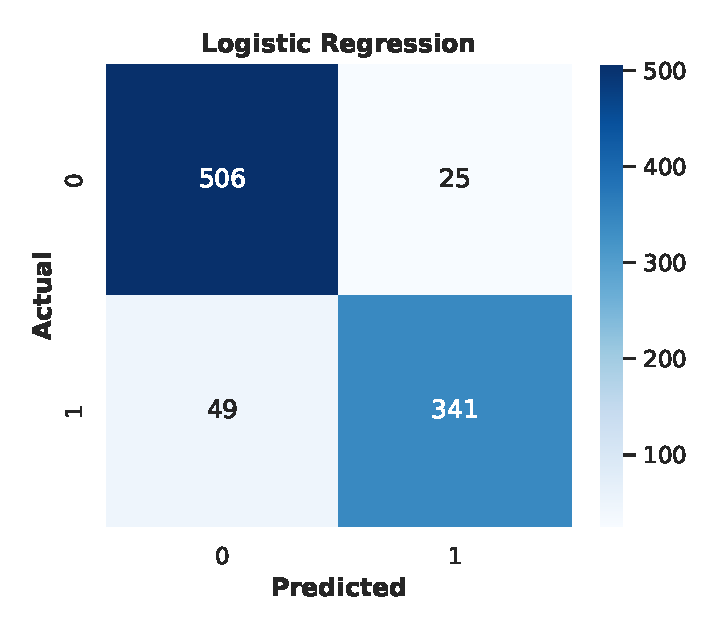
\includegraphics[width=0.5\linewidth]{figures/logistic_confusion_matrix.eps}
\caption{Confusion matrix for the baseline Logistic Regression classifier on the test set.}\label{fig:lr-cm}
\end{figure}
 
\textbf{Inference:}
From Figure~ \ref{fig:lr-cm} we can see Logistic Regression correctly separates the
large majority of both classes, with more false negatives (spam predicted as ham)
than false positives (ham predicted as spam). This matches the recall/precision gap
we saw in Section 8.1 (recall 0.874 vs.\ precision 0.932): the model is more
conservative about labeling an email as spam than about labeling it as ham. In a real
deployment that would mean fewer legitimate emails getting wrongly filtered out, at
the cost of a few more spam emails slipping through. For a spam filter, that's often
the trade-off you actually want, since losing a genuine email (false positive) is
usually more costly to a user than the occasional spam message reaching the inbox
(false negative).
 
\begin{figure}[H]
\centering
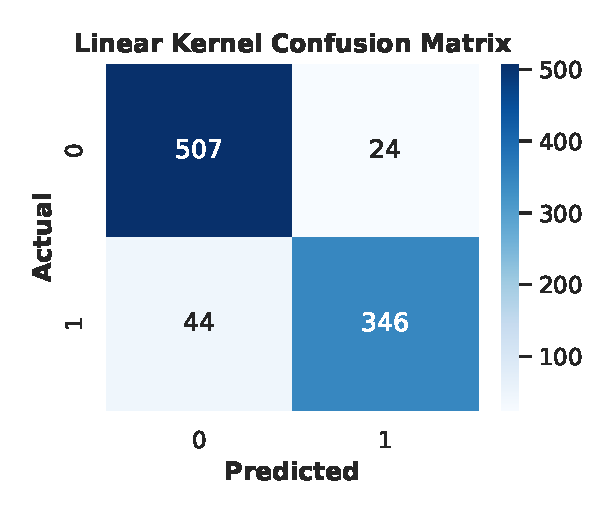
\includegraphics[width=0.42\linewidth]{figures/linear_kernel_confusion_matrix.eps}
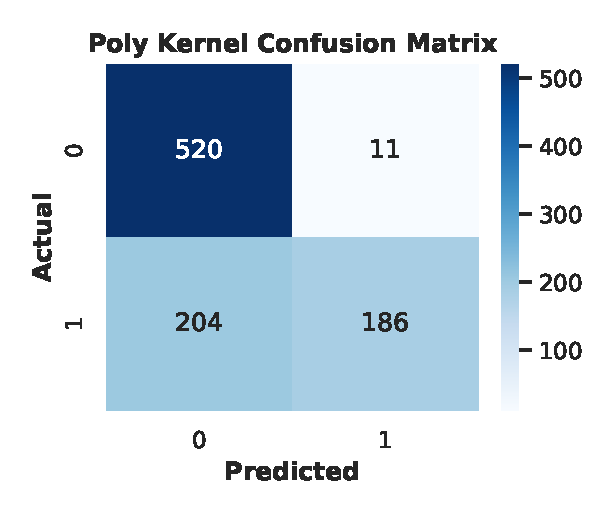
\includegraphics[width=0.42\linewidth]{figures/poly_kernel_confusion_matrix.eps}
\caption{Confusion matrices for the Linear (left) and Polynomial (right) SVM kernels.}\label{fig:svm-cm-1}
\end{figure}
 
\begin{figure}[H]
\centering
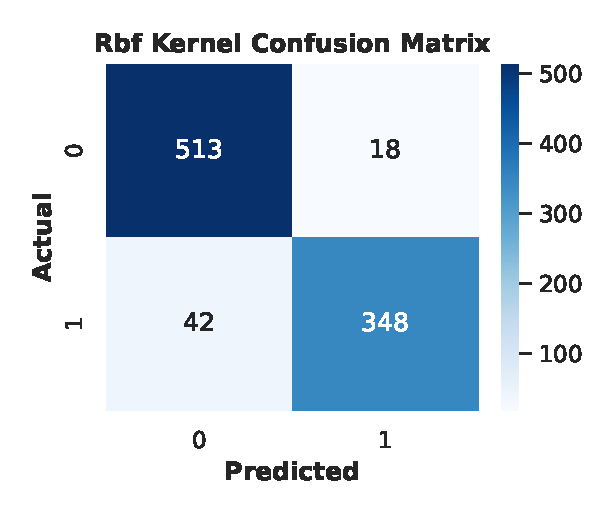
\includegraphics[width=0.42\linewidth]{figures/rbf_kernel_confusion_matrix.eps}
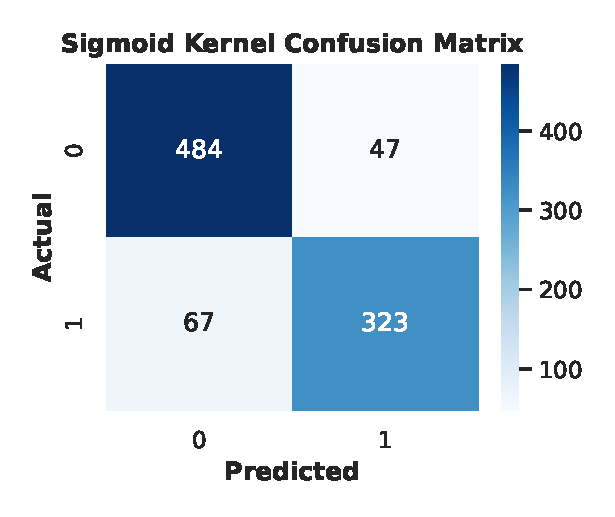
\includegraphics[width=0.42\linewidth]{figures/sigmoid_kernel_confusion_matrix.eps}
\caption{Confusion matrices for the RBF (left) and Sigmoid (right) SVM kernels.}\label{fig:svm-cm-2}
\end{figure}
 
\textbf{Inference:}
Across the four kernel confusion matrices, RBF makes the fewest total errors (18
false positives + 42 false negatives), with the linear kernel close behind (24 + 44).
The polynomial kernel is a clear outlier here -- 204 false negatives, meaning more
than half of all actual spam emails got misclassified as ham -- which drags its
accuracy down to 76.66\% and its F1-score down to 0.634, way below every other kernel.
One likely explanation is that the default polynomial degree (3), combined with the
standardized 57-dimensional feature space, produced a decision boundary that
under-fit the spam class, rather than the polynomial kernel being a genuinely poor
choice in principle. A narrower degree/$\gamma$ search specifically for the
polynomial kernel might close some of that gap. The sigmoid kernel sits in between,
correctly identifying most spam but with a visibly higher false-positive count (47)
than RBF or linear.
 
\begin{figure}[H]
\centering
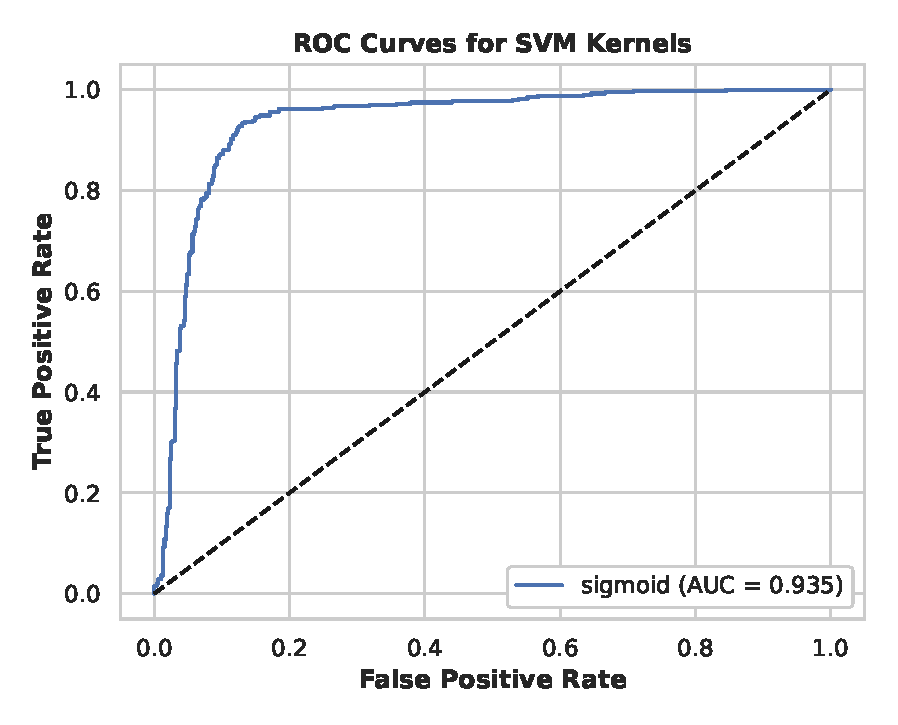
\includegraphics[width=0.65\linewidth]{figures/svm_kernel_roc_curves.eps}
\caption{ROC curves for all four SVM kernels, evaluated on the test set.}\label{fig:svm-roc}
\end{figure}
 
\textbf{Inference:}
The ROC curves in Figure~ \ref{fig:svm-roc} rank the kernels consistently with the
accuracy/F1 table: RBF and linear trace curves closest to the top-left corner
(highest AUC), sigmoid sits slightly below them, and polynomial is visibly the
worst-performing curve, sitting closest to the diagonal no-skill line. So the
polynomial kernel's weakness isn't just an artifact of the default 0.5 decision
threshold -- its ranking of spam-vs-ham probabilities is genuinely less separable
than the other three kernels across all thresholds. The near-overlap between the RBF
and linear curves also points to something interesting: for this particular feature
space, the extra non-linear flexibility of RBF only buys a marginal ranking
improvement over a simple linear separator, which suggests most of the separability
in the Spambase features is already close to linear to begin with.
 
\begin{figure}[H]
\centering
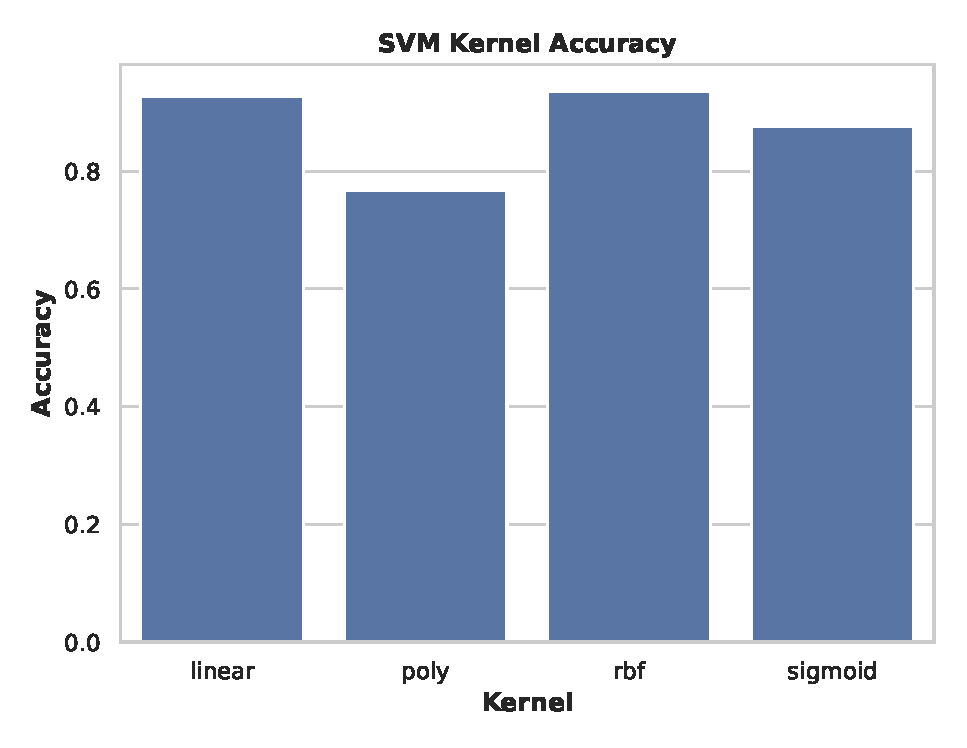
\includegraphics[width=0.55\linewidth]{figures/svm_kernel_accuracy.eps}
\caption{Test accuracy comparison across the four SVM kernels.}\label{fig:svm-bar}
\end{figure}
 
\textbf{Inference:}
The bar chart makes the polynomial kernel's underperformance immediately obvious next
to the other three, which cluster much closer together (87.6\%--93.5\%). RBF has the
tallest bar, just barely ahead of linear, which lines up with \texttt{GridSearchCV}'s
choice (Section 9) of RBF as the best overall kernel. It's a nice sanity check, too --
the grid search's numeric pick (RBF, $C=1$, $\gamma$=scale) matches what you'd see just
from eyeballing the raw per-kernel comparison, rather than being the product of one
lucky cross-validation fold.
 
\begin{figure}[H]
\centering
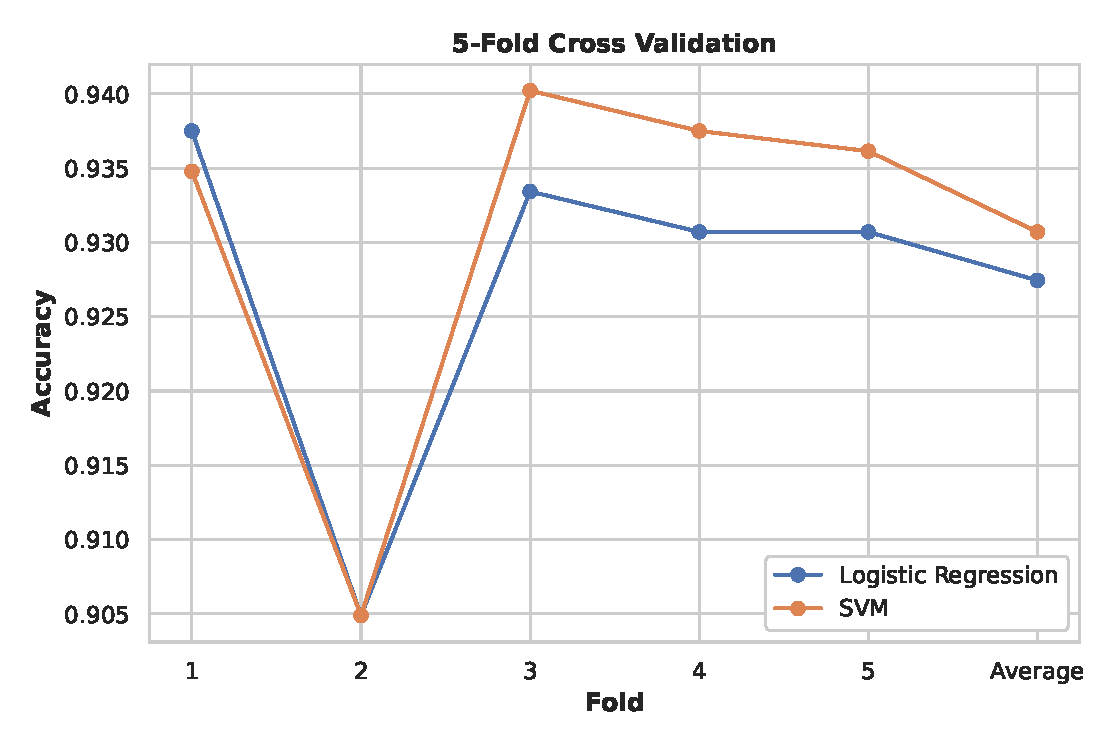
\includegraphics[width=0.65\linewidth]{figures/cross_validation.eps}
\caption{5-fold cross-validation accuracy per fold for the tuned Logistic Regression and SVM models.}\label{fig:cv-plot}
\end{figure}
 
\textbf{Inference:}
Both models show an identical dip at Fold 2 (accuracy drops to 0.905 for both). One
possible explanation is that this particular training fold contains a subset of
emails that are just intrinsically harder to classify (borderline word-frequency
patterns, maybe), rather than either model having some specific weakness -- a
model-specific issue wouldn't hit both algorithms identically on the same fold.
Outside of Fold 2, SVM sits consistently at or slightly above Logistic Regression
(Folds 1, 3, 4, 5), which is why its average CV accuracy (0.9307) edges out Logistic
Regression's (0.9274). The spread across folds for both models is fairly small
(roughly 0.90--0.94), which tells us neither model is especially sensitive to which
80\% of the training data it happens to see -- both generalize with reasonably low
variance.
 
\section{Discussion}
 
\textbf{Best-performing classifier:} The tuned SVM with an RBF kernel got the highest
test accuracy (93.49\%) and the highest 5-fold CV accuracy (93.07\%), narrowly ahead
of the tuned Logistic Regression (91.64\% test accuracy, 92.74\% CV accuracy). The gap
is small -- roughly 1.9 percentage points on the held-out test set -- so which one
actually makes sense to deploy depends a lot on what constraint you're optimizing for.
 
\textbf{Impact of regularization:} Grid Search picked $\ell_1$ regularization with a
comparatively weak penalty ($C=10$) for Logistic Regression. Given how close to zero
the pairwise correlations were in the EDA heatmap, most of the 57 features carry at
least some independent signal, so a weak penalty that keeps nearly all features
(while zeroing out only the least useful ones) generalized better in cross-validation
than a stronger penalty would have. This fits with the roughly 0.7-percentage-point
gap between the untuned baseline Logistic Regression (91.97\% test accuracy, default
$C=1$, L2) and the tuned model's cross-validated score (92.74\%) -- tuning mostly
changed \emph{which} features got kept, not how aggressively the model was
constrained.
 
\textbf{Kernel behaviour in SVM:} The four kernels produced a pretty wide spread in
performance (76.66\%--93.49\% accuracy), which shows kernel choice matters far more
for this dataset than the L1/L2 choice mattered for Logistic Regression. RBF and
linear performed similarly well, which suggests the classes are close to linearly
separable in the standardized feature space, with RBF only providing a small
non-linear refinement on top. The polynomial kernel's collapse in recall (lots of
spam emails misclassified as ham) suggests its fixed-degree expansion distorted the
feature space in a way that made the spam class harder to separate, not easier.
 
\textbf{Bias--variance trade-off:} Logistic Regression, being a linear model with
strong regularization options, sits toward the higher-bias/lower-variance end of the
spectrum -- fast to train (0.03\,s) and stable across folds (the std across the 5
folds is small), but capped in accuracy by its linear decision boundary. SVM with the
RBF kernel sits toward the lower-bias/higher-variance end -- its non-linear boundary
got the best accuracy, but at roughly 50--90$\times$ the training time of Logistic
Regression, along with a noticeably higher-variance dependence on kernel choice, as
the polynomial-kernel results make pretty clear. The cross-validation plot's similar
per-fold shape for both models suggests that once the RBF kernel is actually
selected, its variance is well controlled by the moderate $C=1$ chosen during tuning.
 
\section{Conclusion}
Both Logistic Regression and Support Vector Machines were trained, tuned, and
evaluated on the Spambase dataset without major issues. After 5-fold grid-search
tuning, the RBF-kernel SVM ($C=1$, $\gamma$=scale) delivered the best overall test
accuracy (93.49\%) and F1-score (0.9206), narrowly ahead of the L1-regularized
Logistic Regression ($C=10$, 91.64\% test accuracy). That said, Logistic Regression
trained roughly 20$\times$ faster than even the quickest SVM kernel (RBF, 1.68\,s) and
stays substantially easier to interpret through its learned coefficients. The
polynomial SVM kernel was clearly a poor fit for this dataset without further tuning
of its own degree/$\gamma$ parameters, underperforming every other model by a wide
margin. Overall, for a production spam filter where raw accuracy is the priority, the
tuned RBF-SVM is the better pick; where training/inference speed, interpretability, or
frequent retraining matter more, the tuned Logistic Regression is the stronger
practical choice.
 
\section{References}
\begin{enumerate}
\item scikit-learn developers, ``Logistic Regression,'' scikit-learn User Guide.
[Online]. Available: \\ \url{https://scikit-learn.org/stable/modules/linear_model.html#logistic-regression}
\item scikit-learn developers, ``Support Vector Machines,'' scikit-learn User Guide.
[Online]. Available: \url{https://scikit-learn.org/stable/modules/svm.html}
\item scikit-learn developers, ``Tuning the hyper-parameters of an estimator,''
scikit-learn User Guide. [Online]. Available: \url{https://scikit-learn.org/stable/modules/grid_search.html}
\item Somesh, ``Spambase Dataset,'' Kaggle. [Online]. Available:
\url{https://www.kaggle.com/datasets/somesh24/spambase}
\item M. Hopkins, E. Reeber, G. Forman, and J. Suermondt, ``Spambase,'' UCI Machine
Learning Repository, 1999. [Online]. Available: \url{https://archive.ics.uci.edu/dataset/94/spambase}
\end{enumerate}
 
\end{document}